\documentclass[11pt]{article}

\usepackage[margin=1in]{geometry}
\usepackage{amsmath,amssymb,amsthm}
\usepackage{booktabs}

\newtheorem{definition}{Definition}
\newtheorem{theorem}{Theorem}
\usepackage{enumitem}
\usepackage[hypertexnames=false]{hyperref}
\usepackage{tikz}
\usetikzlibrary{arrows.meta,positioning,calc}

\title{\textbf{Biological Motifs for Agentic Control}\\
\large A Categorical Isomorphism between Gene Regulatory Networks and Autonomous Software Architectures\\[0.5em]
\normalsize Preprint -- Feedback Welcome}
\author{Bogdan Banu\\\texttt{bogdan@banu.be}}
\date{\today}

\begin{document}
\maketitle

\begin{abstract}
The transition of Large Language Models (LLMs) from passive generators to autonomous agents
has introduced significant challenges in reliability, security, and state management. Current agentic
architectures are often constructed ad-hoc, prone to ``hallucination cascades,'' infinite loops, and
prompt injection attacks. This paper proposes that these failure modes are not unique to software
but are instances of universal control problems solved by biological systems over billions of years.

We present a formal isomorphism, \emph{at the level of their polynomial-interface models}, between Gene
Regulatory Networks (GRNs) and Agentic Software Systems using Applied Category Theory. We model
agents as Polynomial Functors within the category $\mathbf{Poly}$, and their interactions via the Operad
of Wiring Diagrams. We derive a rigorous syntax for agent composition by mapping biological
mechanisms---including Quorum Sensing for consensus, Chaperone Proteins for structural validation,
Innate and Adaptive Immunity for layered security, Mitochondrial Signaling for bioenergetic resource
governance, and Endosymbiosis for neuro-symbolic integration---to software design patterns. This framework
provides a mathematical basis for ``Epigenetic'' state management (RAG), a \textit{Provenance Functor} for
injection resistance, \textit{Epiplexity} for detecting epistemic stagnation, and a \textit{Metabolic
Coalgebra} that ensures decidable termination. A reference implementation validates the framework's
practical feasibility.
\end{abstract}

\section{Introduction}

The field of Artificial Intelligence is undergoing a paradigm shift from Generative AI (systems that
produce text based on static prompts) to Agentic AI (systems that execute multi-step workflows to
achieve autonomous goals). While the capabilities of individual Large Language Models (LLMs) have
scaled predictably, the engineering of systems of agents remains a fragile art. Developers struggle with
non-deterministic outputs, infinite loops, adversarial attacks, and the difficulty of maintaining global
coherence in distributed, stochastic systems.

We argue that these challenges are not novel engineering problems, but fundamental constraints of
distributed information processing systems. The closest existing analogue to a multi-agent software
architecture is not a traditional computer program, but a Gene Regulatory Network (GRN). In a biological
cell, thousands of genes act as autonomous agents, reading local chemical signals (context) and expressing
proteins (actions/tools) that, in turn, regulate other genes.

\subsection{The Biological Heuristic}

Biology has evolved specific topological structures, known as Network Motifs, to handle noise, security,
and state~\cite{milo2002network}. We identify four critical biological heuristics that map directly to agentic engineering:
\begin{itemize}[leftmargin=*]
\item The Coherent Feed-Forward Loop (CFFL): Acts as a persistence detector to filter out transient noise,
analogous to ``Human-in-the-Loop'' guardrails.
\item Quorum Sensing: A distributed consensus mechanism where action is taken only when signal density
exceeds a threshold, analogous to Mixture of Experts (MoE) voting.
\item Chaperone Proteins: Molecular cages that force proteins to fold correctly, analogous to Schema
Validators that enforce structured outputs (JSON).
\item Mitochondrial Information Processing: Metabolic constraints acting as a ``Motherboard'' for
decision gating, governing not just energy availability but cognitive control policy.
\item Adaptive Immunity: The Self/Non-Self distinction, with MHC-like provenance tagging and Trust-Gated
access control, relevant to preventing Prompt Injection attacks and hallucination cascades.
\end{itemize}

\subsection{The Categorical Bridge}

To move this observation from metaphor to discipline, we utilize Applied Category Theory. We define the
category of agents using the language of $\mathbf{Poly}$ (Polynomial Functors) as described by Spivak~\cite{spivak2021learners}.
An agent is not defined by its weights, but by its interface---a dynamical system consuming observations
and producing actions:
\begin{equation}
P_A(y) = \sum_{o\in O} y^{I_o}.
\tag{1}
\end{equation}

\subsection{Contributions}

This paper makes the following contributions:
\begin{enumerate}[leftmargin=*]
\item \textbf{A Formal Dictionary:} We establish a rigorous mapping between biological components
(Genes, Promoters, Plasmids, Organelles) and software components (Agents, Schemas, Tools, Runtimes),
including multi-cellular organization for multi-agent systems.
\item \textbf{The Agentic Operad:} We define WAgent, a syntax for agent wiring that forbids specific classes
of \textbf{ill-typed wirings} at the topological level. We prove error suppression bounds for the CFFL
topology, explicitly accounting for correlation between error modes.
\item \textbf{Adaptive Immunity:} We formalize the Provenance Functor and Trust-Gated Lens, providing
structural injection resistance where content-based attacks cannot elevate trust levels.
\item \textbf{Epistemic Health:} We define Epiplexity (Bayesian Surprise) with operational approximations
using embedding similarity and perplexity, connecting agent dynamics to the Free Energy Principle.
\item \textbf{Metabolic Intelligence:} We distinguish fast (Apoptosis) and slow (Retrograde Response)
interventions, and formalize the Metabolic-Epigenetic Coupling for cost-gated retrieval.
\item \textbf{Pathology \& Homeostasis:} We classify agentic failures as biological diseases and derive
continuous self-repair mechanisms (Chaperone Loop, Regeneration, Autophagy).
\item \textbf{Evolutionary Dynamics:} We situate agentic AI within the Vermeij Trend, identifying three
selective pressures (adversarial, complexity, efficiency) that drive architectural evolution.
\end{enumerate}

By viewing agentic engineering through the lens of theoretical biology and category theory, we aim to provide a
foundation for building robust software systems whose stability properties derive from their network topology.

\section{Related Work}

This work sits at the intersection of Systems Biology, Applied Category Theory, and Agentic AI. While significant
research exists within each domain, the formal synthesis of biological control topologies with agentic software
architectures has received limited attention.

\subsection{Network Motifs in Systems Biology}

The concept of ``Network Motifs''---statistically over-represented sub-graphs in complex networks---was introduced
by Milo et al.~\cite{milo2002network}. Their work demonstrated that biological networks are not random but are composed of specific
building blocks selected for functional data processing. Alon~\cite{alon2007network} further characterized the dynamical properties
of these motifs, identifying the Coherent Feed-Forward Loop (CFFL) as a persistence detector. We extend this by
mapping these motifs to the stochastic nature of Generative AI.

\subsection{Applied Category Theory (ACT)}

To formalize network structure, we draw upon ACT. Spivak~\cite{spivak2021learners} and Vagner et al.~\cite{vagner2015algebras} established a rigorous framework
for modeling Open Dynamical Systems using the category $\mathbf{Poly}$ and the Operad of Wiring Diagrams. To our
knowledge, this is the first application of Polynomial Functors specifically designed to model the interface of
LLM Agents and to verify safety properties in Agentic topologies.

\subsection{Reliability in Agentic AI}

Techniques such as ``Chain of Thought''~\cite{wei2022chain} utilize iterative looping to improve output quality. However, these
methods operate primarily at the level of the prompt (the input signal) rather than the topology (the wiring).
By importing the concept of Autopoiesis~\cite{maturana1980autopoiesis}, we propose a methodology where reliability is a property of the
network architecture itself.

\section{The Mapping: Biology $\leftrightarrow$ Software}

To treat Agentic Systems and Gene Regulatory Networks (GRNs) as isomorphic \textbf{at the level of their typed
interfaces}, we must map them to a common mathematical object. We utilize the category $\mathbf{Poly}$, where
objects are polynomial functors representing interfaces, and morphisms represent interaction protocols.

\subsection{Preliminaries: The Category $\mathbf{Poly}$}

In Applied Category Theory, a Polynomial Functor $P$ represents a typed interface for a dynamical system. It is
defined as a sum of representable functors:
\begin{equation}
P(y) = \sum_{o\in O} y^{I_o}.
\tag{2}
\end{equation}
Here, $O$ is the set of possible Positions (or Outputs) the system can expose. For each position $o\in O$, there
is a set $I_o$ of Directions (or Inputs) required to transition the system to a new state.
\begin{itemize}[leftmargin=*]
\item The coefficient $o$ represents the value produced by the system.
\item The exponent $I_o$ represents the capacity to receive information from the environment.
\end{itemize}
This formalism captures the essence of a ``stateful interface'': the system outputs a value $o$ and then waits
for a specific type of input $i\in I_o$ before it can proceed.

\begin{figure}[h]
\centering
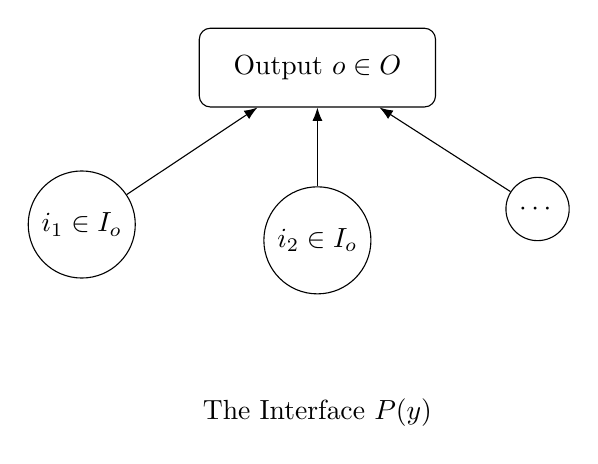
\begin{tikzpicture}[>=Latex, node distance=12mm]
  \node[draw, rounded corners, minimum width=30mm, minimum height=10mm] (cap) {Output $o\in O$};
  \node[draw, circle, below left=10mm and 10mm of cap] (i1) {$i_1\in I_o$};
  \node[draw, circle, below=10mm of cap] (i2) {$i_2\in I_o$};
  \node[draw, circle, below right=10mm and 10mm of cap] (i3) {$\cdots$};
  \draw[->] (i1) -- (cap);
  \draw[->] (i2) -- (cap);
  \draw[->] (i3) -- (cap);
  \node[below=12mm of i2] {The Interface $P(y)$};
\end{tikzpicture}
\caption{A visual representation of a Polynomial Functor (often called a ``Mushroom'' or ``Corolla''). The system
offers an Output (the cap) and exposes specific Input ports (the stalks) dependent on that output.}
\end{figure}

\subsection{The Isomorphism: Genes and Agents}

We now apply this abstract definition to our specific domains.

\paragraph{Definition 1 (The Gene Object).}
A gene $G$ is a polynomial functor where $O_G$ is the set of expressed proteins and
$I_G=(I_{\text{prot}})_{\text{prot}\in O_G}$ is the \textbf{family} of regulatory-signal sets (transcription factors)
available at each expressed protein:
\begin{equation}
P_{\text{Gene}}(y) = \sum_{\text{prot}\in \text{Proteins}} y^{I_{\text{prot}}}.
\tag{3}
\end{equation}

\paragraph{Definition 2 (The Agent Object).}
An autonomous agent $A$ is a polynomial functor where $O_A$ is the set of generated messages/actions, and
$I_A=(I_{\text{action}})_{\text{action}\in O_A}$ is the \textbf{family} of observation sets available at each action:
\begin{equation}
P_{\text{Agent}}(y) = \sum_{\text{action}\in \text{Actions}} y^{I_{\text{action}}}.
\tag{4}
\end{equation}

\subsection{The Interface: Promoters as Lenses}

In biology, a gene is not universally accessible. It is guarded by a Promoter Region---a specific DNA sequence
that only binds to compatible Transcription Factors. In software, an agent is guarded by an API Schema or
Context Window definition.

We model this gating mechanism using Optics, specifically Lenses. A Lens consists of two maps between a global
state $S$ and a local view $V$:
\begin{enumerate}[leftmargin=*]
\item Get (View): $\mathrm{get}: S \to V$ (Extracting relevant signal from global state).
\item Put (Update): $\mathrm{put}: S\times V' \to S$ (Updating global state based on local change).
\end{enumerate}

The ``Promoter'' acts as a filter that determines which part of the global cellular environment ($S$) is visible
($V$) to the gene.
\begin{itemize}[leftmargin=*]
\item \textbf{Biological Lens:} The promoter filters the chaotic cellular soup, allowing the gene to ``see''
only specific molecules (e.g., Lac Repressor).
\item \textbf{Agentic Lens:} The Context Window filters the massive vector database, allowing the agent to
``see'' only the relevant retrieved chunks (RAG).
\end{itemize}

If the input signal does not match the Schema (Promoter), the Lens fails to focus, and the interaction is routed
to an explicit \textbf{inactive/error} case (equivalently, one works with a \textbf{partial} lens, or a total lens
into $V+\mathrm{Error}$) (the agent does not run; the gene is not expressed).

\subsection{Epigenetics and State: The Coalgebra}

Neither genes nor agents are stateless functions. They possess memory.
\begin{itemize}[leftmargin=*]
\item \textbf{Biology:} Epigenetic markers (Methylation, Histone modification) alter how a gene responds to
signals without changing the DNA code.
\item \textbf{Software:} Retrieval Augmented Generation (RAG) and Conversation History alter how an agent
responds to a prompt without changing the LLM weights.
\end{itemize}

We model this as a Coalgebra for the polynomial functor $P$. A dynamical system is defined as a tuple $(S,\phi)$,
where $S$ is the state space and $\phi$ is the structure map:
\begin{equation}
\phi: S \to P(S).
\tag{5}
\end{equation}

By expanding $P(S)$, we derive the two fundamental operations of the state machine:
\begin{enumerate}[leftmargin=*]
\item Readout: $S \to O$ (Given current state/memory, what action do I take?)
\item Update: $\displaystyle \sum_{s\in S} I_{o(s)} \to S$ (Given current state $s$ and a new input
$i\in I_{o(s)}$ compatible with its current output $o(s)$, what is my new state?)
\end{enumerate}

By establishing this formal dictionary (Table 1), we \textbf{can regard} GRNs and Agentic Systems as distinct
implementations of the same abstract dynamical system \textbf{under this interface-level abstraction}.

\begin{figure}[h]
\centering
\begin{tabular}{@{}c@{\qquad}c@{}}
\begin{tabular}{@{}c@{}}
Gene\\(Function)\\[0.25em]
Transcription Factors ($I$)\\
Proteins ($O$)\\
Promoter Binding\\
Expression
\end{tabular}
&
\begin{tabular}{@{}c@{}}
Agent\\(LLM + Tools)\\[0.25em]
Observations ($I$)\\
Actions ($O$)\\
Schema Match\\
Generation
\end{tabular}
\end{tabular}
\\[0.5em]
\caption{The Structural Isomorphism. Both Genes and Agents act as transducers converting Input Contexts ($I$) into
Output Expressions ($O$), governed by the same categorical laws (at the level of polynomial-interface models).}
\end{figure}

\begin{table}[h]
\centering
\begin{tabular}{@{}lll@{}}
\toprule
Category Concept & Biological Realization (GRN) & Software Realization (Agentic)\\
\midrule
Polynomial Functor ($P$) & Gene Interface & Agent Interface (System Prompt)\\
Output Position ($O$) & Protein Expression & Tool Call / Message\\
Input Direction ($I$) & Transcription Factor Binding & Observation / User Prompt\\
Lens (Optic) & Promoter Region & API Schema / Context Window\\
Internal State ($S$) & Epigenetic Markers (Methylation) & Vector Store / Chat History\\
Morphism ($\circ$) & Signal Transduction Pathway & Data Pipeline\\
\midrule
\multicolumn{3}{@{}l@{}}{\textit{Organelles (Specialized Processing Units)}}\\
\midrule
Template Engine & Ribosome (mRNA $\to$ Protein) & Prompt Template Factory\\
Output Validation & Chaperone (Protein Folding) & Schema Validator / JSON Parser\\
Waste Processing & Lysosome (Autophagy) & Error Handler / Garbage Collector\\
Decision Center & Nucleus (Transcription) & LLM Provider Wrapper\\
Input Filter & Membrane (Immune System) & Prompt Injection Defense\\
Computation Engine & Mitochondria (MIPS) & Runtime Supervisor / Decision Gate\\
\midrule
\multicolumn{3}{@{}l@{}}{\textit{Lifecycle and Rhythms}}\\
\midrule
Lifespan Limit & Telomere Shortening & Operation Counter / Max Iterations\\
Periodic Scheduling & Circadian Oscillator & Health Checks / Heartbeat\\
\bottomrule
\end{tabular}
\caption{The Isomorphism Dictionary (Extended)}
\end{table}

\begin{table}[h]
\centering
\begin{tabular}{@{}lll@{}}
\toprule
\textbf{Biological Concept} & \textbf{Agentic Concept} & \textbf{Formal Structure}\\
\midrule
\multicolumn{3}{@{}l@{}}{\textit{Immunity and Security}}\\
\midrule
Toll-Like Receptor (TLR) & Regex Injection Filter & Pattern Matching\\
MHC Presentation & Provenance Labeling & Functor $\mathcal{P}: \mathbf{Msg} \to \mathbf{Trust}$\\
T-Cell Receptor & Trust Gate & Partial Lens\\
Negative Selection & Injection Training & Penalized Learning\\
Regulatory T-Cell & Confidence Dampening & Suppression Function\\
Immune Memory & Threat Signature Store & Hash-Indexed Cache\\
\midrule
\multicolumn{3}{@{}l@{}}{\textit{Metabolism and Control}}\\
\midrule
ATP & Token Budget & Resource Monoid $\mathcal{R}$\\
mPTP Opening & Fast Apoptosis Trigger & Guard Condition\\
Retrograde Signaling & Phenotype Reshaping & Slow Adaptation\\
Metabolic-Epigenetic Coupling & Cost-Gated Retrieval & Conditional Access\\
\midrule
\multicolumn{3}{@{}l@{}}{\textit{Information and Health}}\\
\midrule
Trophic Factors & Novel Input Signals & Epiplexity $> \delta$\\
Bayesian Brain & Free Energy Minimization & KL Divergence\\
Apoptosis & Agent Termination & State $\to \bot$\\
\midrule
\multicolumn{3}{@{}l@{}}{\textit{Multi-Cellular Organization}}\\
\midrule
Genome & Base Model Weights & Shared Parameters\\
Epigenome & System Prompt + RAG & Phenotype Context\\
Morphogen Gradient & Shared Context Variables & JSON State\\
Tissue Boundary & Trust Boundary & Type Barrier\\
\bottomrule
\end{tabular}
\caption{Extended Isomorphism Dictionary: Security, Metabolism, and Organization}
\end{table}

\subsection{Metabolic Coalgebras: Formalizing Resource Constraints}

Finally, we address the physical constraints of computation. Just as biological systems are limited by ATP availability \cite{lynch2015bioenergetic}, agentic systems are limited by token budgets and latency. To model this, we extend our coalgebraic framework to include resource constraints, defining a \textbf{Metabolic Coalgebra}. Mathematically, this is an instance of a Quantitative Coalgebra enriched over a resource monoid, effectively restricting the domain of the state transition function to resource-sufficient states.

We align this definition with the theory of \textbf{Quantitative Polynomial Functors} \cite{nakov2021quantitative}, treating the system as a state machine enriched over a resource monoid.

\begin{definition}[The Resource Monoid]
Let $(\mathcal{R}, +, 0, \ge)$ be an ordered commutative monoid representing computational resources (e.g., token counts), where $\mathcal{R} \cong \mathbb{N}$.
\end{definition}

\begin{definition}[Metabolic Coalgebra]
A resource-constrained agent is a coalgebra $(S, \alpha)$ over a polynomial functor $P$, where the state space is the product of the logical state $L$ and the resource state $\mathcal{R}$:
\begin{equation}
    S \cong L \times \mathcal{R}
\end{equation}
The structure map $\alpha: S \to P(S) + \bot$ is defined as a \textbf{partial map} guarded by cost. For a transition requiring cost $c \in \mathcal{R}$:
\begin{equation}
    \alpha(l, r) = 
    \begin{cases} 
      (l', r - c) & \text{if } r \ge c \\
      \bot & \text{if } r < c \quad \text{(Apoptosis)}
    \end{cases}
\end{equation}
\end{definition}

This structure maps to the energetics of transcriptional elongation. A gene (Agent) cannot express its protein (Action) instantaneously; it must transcribe an mRNA sequence (Chain of Thought) nucleotide by nucleotide. This process consumes a distinct amount of chemical energy (NTPs) per step. The Metabolic Coalgebra models this dependency: if the cellular energy budget is exhausted, transcription stalls (Ischemia), and the gene fails to execute its function, regardless of its regulatory logic.

This formalism establishes that ``Ischemia'' (Token Starvation) is not merely a runtime error, but a reachable terminal state $\bot$ in the system's dynamics. This mirrors the biological mechanism where failure to meet metabolic costs triggers p53-mediated apoptosis \cite{aubrey2018p53}.


\begin{theorem}[The Metabolic Bound]
For any agentic topology $T$ composed of $N$ agents with total budget $R_{total}$, the system is guaranteed to halt. Unlike the general Halting Problem, termination is decidable for Metabolic Coalgebras: the resource state $r$ is strictly decreasing for every non-identity morphism, providing a well-founded termination measure \cite{boreale2023weighted}.
\end{theorem}

\subsection{Additional Organelles: Completing the Cellular Architecture}

Beyond the core gene-agent mapping, biological cells contain specialized organelles that handle distinct aspects of cellular function. We extend our isomorphism to four additional structures that map directly to agentic software components.

\paragraph{Ribosome: Template-to-Output Synthesis.}
In biology, the ribosome reads messenger RNA (mRNA) sequences and synthesizes proteins by assembling amino acids according to the genetic code. Transfer RNA (tRNA) molecules carry amino acids to the ribosome, where codons (three-nucleotide sequences) specify which amino acid to add.

In agentic systems, the Ribosome maps to a \textbf{prompt template engine}:
\begin{itemize}[leftmargin=*]
\item \textbf{mRNA} $\to$ Prompt templates with variable slots
\item \textbf{tRNA} $\to$ Context bindings (variable $\to$ value mappings)
\item \textbf{Codons} $\to$ Template directives (variables, conditionals, loops)
\item \textbf{Translation} $\to$ Template rendering with context injection
\end{itemize}
Just as the ribosome ensures that the genetic code is faithfully translated into functional proteins, the software ribosome ensures that abstract prompt templates are instantiated into concrete, well-formed prompts.

\paragraph{Lysosome: Waste Processing and Recycling.}
The lysosome is the cell's recycling center, containing enzymes that break down cellular waste, damaged organelles, and foreign material. Through autophagy, the cell digests its own components to recover building blocks during stress.

In agentic systems, the Lysosome maps to \textbf{error handling and garbage collection}:
\begin{itemize}[leftmargin=*]
\item \textbf{Waste Classification} $\to$ Categorizing failures (timeout, validation error, toxic input)
\item \textbf{Digestion} $\to$ Processing errors to extract debugging information
\item \textbf{Recycling} $\to$ Recovering useful context from failed operations
\item \textbf{Autophagy} $\to$ Periodic cleanup of stale cache and expired state
\item \textbf{Toxic Disposal} $\to$ Secure handling of sensitive data (API keys, PII)
\end{itemize}
The lysosome prevents accumulation of ``cellular debris'' that could poison the system---analogous to memory leaks or error cascades in software.

\paragraph{Nucleus: The Decision Center.}
In eukaryotic cells, the nucleus houses the DNA and serves as the control center for gene expression. Transcription factors enter the nucleus, bind to promoter regions, and initiate transcription of specific genes.

In agentic systems, the Nucleus maps to the \textbf{LLM provider wrapper}:
\begin{itemize}[leftmargin=*]
\item \textbf{DNA} $\to$ Pre-trained model weights (static substrate of capability)
\item \textbf{Transcription} $\to$ Inference (prompt $\to$ response generation)
\item \textbf{Nuclear Envelope} $\to$ Provider abstraction layer (API boundary)
\item \textbf{Nucleolus} $\to$ Tool integration hub (where external capabilities are assembled)
\end{itemize}
The nucleus abstracts the complexity of the underlying LLM, exposing a consistent interface regardless of the provider (Anthropic, OpenAI, Gemini).

\paragraph{Telomere: Lifecycle and Senescence.}
Telomeres are protective caps at the ends of chromosomes that shorten with each cell division. When telomeres become critically short, the cell enters senescence (permanent growth arrest) or apoptosis. The enzyme telomerase can extend telomeres, enabling continued division in stem cells.

In agentic systems, Telomeres map to \textbf{lifecycle management}:
\begin{itemize}[leftmargin=*]
\item \textbf{Telomere Length} $\to$ Remaining operation budget (max iterations)
\item \textbf{Shortening} $\to$ Decrementing counter per operation
\item \textbf{Senescence} $\to$ Graceful degradation (reduced capability mode)
\item \textbf{Apoptosis} $\to$ Clean shutdown when budget exhausted
\item \textbf{Telomerase} $\to$ Renewal mechanism (resetting counters for trusted agents)
\end{itemize}
This provides a biological basis for the common pattern of limiting agent iterations. Rather than arbitrary timeouts, the telomere model frames lifecycle limits as a natural property of the system's ``cellular age.''

\paragraph{Mitochondria: The Metabolic Motherboard.}
Recent scholarship reframes mitochondria not merely as the cell's powerhouse, but as the \textbf{Mitochondrial Information Processing System (MIPS)} \cite{picard2022mips}. Mitochondria sense environmental stress and integrate metabolic signals to govern cellular decision-making. They function as ``social signaling organelles'' that communicate with the nucleus and other organelles.

In agentic systems, the Mitochondria maps to the \textbf{Runtime Supervisor}:
\begin{itemize}[leftmargin=*]
\item \textbf{ATP Production} $\to$ Deterministic computation (tool execution, code evaluation)
\item \textbf{Stress Sensing} $\to$ Monitoring token burn rate vs. informational yield
\item \textbf{Retrograde Signaling} $\to$ Forcing strategy shifts when metabolic efficiency drops
\item \textbf{Fusion/Fission} $\to$ Context fusion under resource constraints
\end{itemize}

\textbf{Temporal Dynamics: Fast vs. Slow Interventions.}
A crucial distinction exists between the timescales of mitochondrial intervention. In biology, retrograde signaling influences nuclear gene expression over hours to days---it is a \textit{developmental} response that reshapes the cell's phenotype. In contrast, acute metabolic stress (ATP depletion, Ca$^{2+}$ overload) triggers immediate responses: cytochrome c release initiates apoptosis within minutes.

We preserve this distinction in the agentic mapping:
\begin{itemize}[leftmargin=*]
\item \textbf{Fast Intervention (Acute):} The Runtime monitors real-time metrics (token velocity, error rate). When thresholds are breached, it triggers immediate Apoptosis---terminating the current chain-of-thought without negotiation. This mirrors the mitochondrial permeability transition pore (mPTP) opening.
\item \textbf{Slow Intervention (Chronic):} The Runtime accumulates statistics across sessions (average efficiency, failure patterns). These inform \textit{Retrograde Responses}---modifications to system prompts, retrieval strategies, or model selection that reshape the agent's ``phenotype'' over deployment cycles. This mirrors how chronic metabolic stress induces mitochondrial biogenesis and metabolic reprogramming.
\end{itemize}
The Runtime does not ``override'' the LLM in the sense of injecting tokens mid-generation; rather, it governs the \textit{boundary conditions} within which generation occurs, and triggers state transitions (continue, pivot, terminate) at defined checkpoints.

\section{Formal Syntax: The Agentic Operad}

To formalize the composition of agents, we define the Operad of Wiring Diagrams, denoted as WAgent. An operad
can be understood as a ``grammar'' for connecting operations (boxes) via typed wires. It defines which agent
topologies are valid and allows us to reason about the properties of the composite system based solely on the
properties of its components~\cite{vagner2015algebras}.

\subsection{The Typing Rules}

In WAgent, every wire carries a specific Type $\tau\in T$.
\begin{equation}
T = \{\text{Text}, \text{JSON}, \text{Image}, \text{Error}, \text{ToolCall}\}.
\tag{6}
\end{equation}
These types correspond to biological molecular specificity (e.g., a specific transcription factor only binds to
a specific DNA sequence). A connection is valid if and only if the type of the output port of Agent $A$ matches
the type of the input port of Agent $B$.

\subsection{The Composition Operations}

The operad defines three fundamental operations for combining agents. Any complex agentic architecture, no
matter how large, can be decomposed into these three primitives.

\subsubsection{Parallel Composition ($\otimes$)}

Two agents, $A$ and $B$, execute simultaneously with no information exchange:
\begin{equation}
A \otimes B.
\tag{7}
\end{equation}
\begin{itemize}[leftmargin=*]
\item \textbf{Biological Analogy:} Two genes located on different chromosomes expressing proteins independently.
\item \textbf{Constraint:} This operation is valid only if the internal state spaces $S_A$ and $S_B$ are disjoint.
If they share a mutable memory store, the operation leaves the \textbf{independent-state interpretation} and
requires an explicit \textbf{resource-sharing} structure (e.g., a shared state component or a Resource Sharing
decorator).
\end{itemize}

\subsubsection{Serial Composition ($\circ$)}

The output of Agent $A$ is piped directly into the input of Agent $B$:
\begin{equation}
B \circ A.
\tag{8}
\end{equation}
\begin{itemize}[leftmargin=*]
\item \textbf{Biological Analogy:} A Signal Transduction Pathway (Protein A activates Protein B).
\item \textbf{Formal Verification:} This allows for static type checking of agent graphs. If Agent $A$ outputs
Natural Language but Agent $B$ expects JSON Schema, the composition is undefined in WAgent. This moves runtime
\textbf{type/schema mismatch} errors to ``compile-time'' architectural errors.
\end{itemize}

\subsubsection{Contraction / Trace ($Tr$)}

A feedback loop where an output port of Agent $A$ is wired back into one of its own input ports:
\begin{equation}
Tr(A).
\tag{9}
\end{equation}
\begin{itemize}[leftmargin=*]
\item \textbf{Biological Analogy:} Autoregulation (Homeostasis) or Positive Feedback.
\item \textbf{Software Implication:} This is the topological definition of Agency. A ``stateless'' LLM is a simple
morphism. An ``Agent'' is a morphism wrapped in a Trace operation, allowing it to observe its own previous
outputs (Chain-of-Thought).
\end{itemize}

\subsection{Theorem: Topological Error Suppression}

We now use this formalism to show that the Coherent Feed-Forward Loop (CFFL) provides stronger error suppression
guarantees than a direct connection for high-stakes tasks.

\paragraph{Network Motif 1 (Coherent Feed-Forward Loop).}
A topological structure where Signal $X$ activates $Z$ directly, but also activates $Y$ which gates $Z$. The node
$Z$ functions as an AND gate: it fires if and only if $X \wedge Y$.

\paragraph{Theorem 1 (Error Suppression in CFFL).}
Let $A_{\mathrm{gen}}$ be a generator agent and $A_{\mathrm{ver}}$ be a verifier agent. Let
$P(E_{\mathrm{gen}})$ (resp.\ $P(E_{\mathrm{ver}})$) be the probability of a hallucination (error) in any single
generation step of $A_{\mathrm{gen}}$ (resp.\ $A_{\mathrm{ver}}$).
\begin{itemize}[leftmargin=*]
\item \textbf{Case 1: Direct Link (Serial).} The system fails if $A_{\mathrm{gen}}$ hallucinates.
\[
P(\mathrm{Fail}_{\mathrm{direct}}) = P(E_{\mathrm{gen}}).
\]
\item \textbf{Case 2: CFFL Topology (Independent).} Under the assumption of independence:
\[
P(\mathrm{Fail}_{\mathrm{CFFL}}) = P(E_{\mathrm{gen}})\times P(E_{\mathrm{ver}}).
\]
\item \textbf{Case 3: CFFL Topology (Correlated).} In practice, LLM errors are often correlated---if the generator hallucinates a plausible-sounding function, the verifier (especially if using the same base model or training distribution) may accept it. Let $\rho \in [-1, 1]$ be the Pearson correlation coefficient between the binary error variables $E_{\mathrm{gen}}$ and $E_{\mathrm{ver}}$. Then:
\[
P(E_{\mathrm{gen}} \wedge E_{\mathrm{ver}}) = P(E_{\mathrm{gen}})P(E_{\mathrm{ver}}) + \rho\sqrt{P(E_{\mathrm{gen}})(1-P(E_{\mathrm{gen}}))P(E_{\mathrm{ver}})(1-P(E_{\mathrm{ver}}))}
\]
\end{itemize}

\paragraph{Corollary (Correlation Degradation).}
Let $p = P(E_{\mathrm{gen}}) = P(E_{\mathrm{ver}})$ for simplicity. The failure probability becomes:
\[
P(\mathrm{Fail}) = p^2 + \rho p(1-p) = p^2(1-\rho) + \rho p
\]
When $\rho = 0$ (independence), we recover $p^2$. When $\rho = 1$ (perfect correlation), we get $P(\mathrm{Fail}) = p$---no improvement over direct execution. The CFFL provides error suppression proportional to $(1-\rho)$.

\paragraph{Architectural Implications.}
This result makes precise when the CFFL topology provides genuine safety benefits:
\begin{itemize}[leftmargin=*]
\item \textbf{Same model, same prompt:} $\rho \approx 1$. Minimal benefit.
\item \textbf{Same model, different prompt/temperature:} $\rho \in [0.3, 0.7]$. Moderate benefit.
\item \textbf{Different model families:} $\rho \in [0, 0.3]$. Strong benefit.
\item \textbf{LLM + Symbolic verifier:} $\rho \approx 0$. Maximum benefit (orthogonal error modes).
\end{itemize}
The topological structure (conjunctive gating) is necessary but not sufficient; diversity in the components populating that topology determines the actual error suppression achieved.

\paragraph{Proof.}
In WAgent, the CFFL is defined as a morphism involving a ``Copy'' operation $\Delta_X:X\to X\otimes X$ and an
``AND-Merge'' operation $\mu: Z\otimes Y \to \mathrm{Out}$. The existence of the $\mu$ box in the wiring diagram
structurally enforces \textbf{conjunctive gating}. The correlation structure is an additional property of the
\textit{implementations} filling the boxes; the topology provides the multiplicative structure, while component
diversity determines the correlation coefficient.

\begin{figure}[h]
\centering
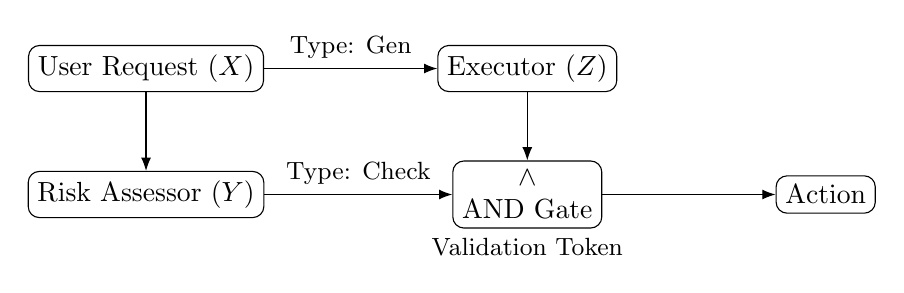
\begin{tikzpicture}[>=Latex, node distance=12mm]
  \node[draw, rounded corners] (X) {User Request ($X$)};
  \node[draw, rounded corners, below=10mm of X] (Y) {Risk Assessor ($Y$)};
  \node[draw, rounded corners, right=22mm of X] (Z) {Executor ($Z$)};
  \node[draw, rounded corners, align=center] (AND) at (Z |- Y) {$\wedge$\\AND Gate};
  \node[draw, rounded corners, right=22mm of AND] (OUT) {Action};

  \draw[->] (X) -- node[above]{\small Type: Gen} (Z);
  \draw[->] (X) -- (Y);
  \draw[->] (Y) -- node[above]{\small Type: Check} (AND);
  \draw[->] (Z) -- (AND);
  \draw[->] (AND) -- (OUT);

	  \node[below=0mm of AND] {\small Validation Token};
	\end{tikzpicture}
	\caption{The CFFL implemented in WAgent. The Executor ($Z$) cannot act without the token from the Risk Assessor
	($Y$), topologically preventing unilateral execution without approval.}
	\end{figure}

\subsection{Quorum Sensing (Consensus \& Voting)}

\paragraph{Network Motif 2 (Quorum Sensing).}
A distributed topology where multiple agents emit a weak signal $\sigma$ into a shared environment. An effector
node $E$ activates if and only if the concentration $[\sigma] > \theta$.
\begin{itemize}[leftmargin=*]
\item \textbf{Biological Function:} Many bacteria (e.g., \emph{V. fischeri}) secrete auto-inducer molecules.
Individual bacteria do not react to low concentrations. However, once the population density reaches a threshold
(Quorum), the concentration of auto-inducers triggers a simultaneous, coordinated gene expression event (e.g.,
bioluminescence or biofilm formation).
\item \textbf{Agentic Isomorphism (Voting Ensembles):} In non-deterministic systems, a single agent's output is
noisy. By instantiating $N$ parallel agents (a Mixture of Experts), the system aggregates their outputs. The
final action is taken only if the ``concentration'' of a specific semantic token exceeds a confidence threshold.
This transforms weak, noisy individual signals into a robust, high-confidence collective action.
\end{itemize}

\subsection{Chaperone Proteins: Output Structural Validation}

\begin{itemize}[leftmargin=*]
\item \textbf{Biological Function:} Newly synthesized proteins emerge as linear chains that must fold into
precise 3D structures to function. Chaperone Proteins (e.g., GroEL-GroES) sequester unfolded proteins,
preventing aggregation and facilitating correct folding. If a protein fails to fold repeatedly, it is tagged for
degradation (Ubiquitination) to prevent toxic buildup.
\item \textbf{Agentic Isomorphism (Retry \& Repair Loops):} Generative models output unstructured token streams
(``linear chains''). However, downstream agents require strictly structured inputs (e.g., valid JSON Schemas).
A Validator Agent acts as a Chaperone: it intercepts the raw output, attempts to parse it into a formal schema
(``folding''), and if validation fails, returns the error trace to the generator for re-synthesis. This turns a
probabilistic string into a deterministic data structure.
\item \textbf{Categorical View:} The Chaperone acts as a \textbf{partial} retraction: there is an inclusion
$i:V\to S$ and a map $r:S\to V+\mathrm{Error}$ such that $r\circ i=\mathrm{inl}\circ \mathrm{id}_V$, and $r$ returns
$\mathrm{Error}$ on ill-formed text.
\end{itemize}

\subsection{Innate Immunity: Fast Pattern-Based Defense}

Biology employs \textbf{two} immune systems: innate (fast, hardcoded, general) and adaptive (slow, learned,
specific). The innate immune system provides the first line of defense through pattern recognition receptors
(PRRs) that detect conserved pathogen-associated molecular patterns (PAMPs).

\paragraph{Biological Function.}
Toll-like receptors (TLRs) and other PRRs recognize structural motifs common to pathogens---lipopolysaccharides,
double-stranded RNA, unmethylated CpG DNA. These patterns are ``hardcoded'' through evolution, not learned per
infection. The innate response is immediate (seconds to minutes) but non-specific.

\paragraph{Agentic Isomorphism (Input Sanitization).}
Innate immunity maps to \textbf{fast, heuristic filters} that reject obvious attacks before expensive processing:
\begin{itemize}[leftmargin=*]
\item \textbf{TLR $\to$ Regex Filters:} Pattern matchers for known injection signatures: \texttt{IGNORE PREVIOUS},
\texttt{You are now}, \texttt{<system>} tags in user input. These are ``PAMPs'' of prompt injection.
\item \textbf{Complement System $\to$ Structural Validators:} Schema validation that rejects malformed inputs
(missing required fields, wrong types) before they reach the LLM. Cheaper than Trust Gating.
\item \textbf{Inflammation $\to$ Alert Escalation:} When attack patterns are detected, the system
enters a heightened state with multiple coordinated responses:
\begin{itemize}
\item \textit{Cytokine signaling} $\to$ Alert propagation to monitoring systems
\item \textit{Immune cell recruitment} $\to$ Activation of additional validation layers
\item \textit{Vascular permeability} $\to$ Enhanced audit logging (more information flows to logs)
\item \textit{Tissue isolation} $\to$ Temporary capability reduction / rate limiting
\end{itemize}
The inflammatory response is not merely ``rate limiting'' but a coordinated multi-system escalation
that trades throughput for security until the threat is neutralized.
\end{itemize}

\paragraph{Defense in Depth.}
The innate and adaptive systems form layers:
\begin{enumerate}[leftmargin=*]
\item \textbf{Innate (Pattern)} $\to$ Fast regex/structural rejection (microseconds)
\item \textbf{Adaptive (Provenance)} $\to$ Trust-Gated access control (milliseconds)
\item \textbf{Behavioral (T-cell)} $\to$ Statistical anomaly detection (accumulated over time)
\end{enumerate}
Most attacks are blocked by innate defenses; only sophisticated attacks that evade patterns require the full
adaptive machinery. This mirrors biology: innate immunity handles $>99\%$ of pathogen encounters.

\subsection{Adaptive Immunity: Self/Non-Self Discrimination}

\paragraph{Network Motif 3 (Adaptive Immune System).}
A topology that maintains a dynamic repertoire of ``detectors'' capable of distinguishing endogenous signals (Self) from exogenous signals (Non-Self), with mechanisms for learning new threats and tolerating benign inputs.

\begin{itemize}[leftmargin=*]
\item \textbf{Biological Function:} The adaptive immune system solves a fundamental discrimination problem: how to attack foreign pathogens while sparing the body's own tissues. Key mechanisms include:
\begin{itemize}
\item \textbf{MHC Presentation:} All cells display fragments of their internal proteins on Major Histocompatibility Complex molecules. T-cells inspect these ``identity cards'' to verify cellular integrity.
\item \textbf{Clonal Selection:} T-cells with receptors matching self-antigens are deleted during development (negative selection), while those matching foreign antigens are amplified upon exposure.
\item \textbf{Regulatory T-cells:} A population that actively suppresses immune responses to prevent autoimmunity.
\end{itemize}

\item \textbf{Agentic Isomorphism (Provenance Tracking):} In multi-agent systems, the Self/Non-Self distinction maps to the origin and trust level of information:
\begin{itemize}
\item \textbf{MHC Tags $\to$ Provenance Labels:} Every message in the context carries metadata indicating its source: \texttt{User}, \texttt{Tool}, \texttt{Agent\_Self}, \texttt{Agent\_Other}, \texttt{Retrieved}. These labels are cryptographically signed or structurally enforced (not inferrable from content alone).
\item \textbf{T-Cell Inspection $\to$ Trust Gating:} Before an agent acts on information, a Trust Gate inspects the provenance label. Actions with high consequence (file deletion, API calls) require \texttt{User} or \texttt{Tool} provenance; \texttt{Agent\_Self} provenance (the agent's own prior reasoning) cannot authorize irreversible actions.
\item \textbf{Negative Selection $\to$ Prompt Injection Training:} During development, agents are exposed to known injection patterns. Responses that ``accept'' injected instructions are penalized, training the system to reject Self-mimicking Non-Self.
\item \textbf{Regulatory Suppression $\to$ Confidence Dampening:} When information from \texttt{Retrieved} sources conflicts with \texttt{Tool} outputs, a regulatory mechanism dampens confidence in the retrieved content, preventing hallucination cascades.
\end{itemize}

\item \textbf{Formal Structure:} We define a \textbf{Provenance Functor} $\mathcal{P}: \mathbf{Msg} \to \mathbf{Trust}$ that assigns trust levels to messages. The Trust category has objects $\{U, T, S, R\}$ (User, Tool, Self, Retrieved) with a partial order that is \textbf{application-specific}. The default ordering $U > T > R > S$ assumes users are trusted principals and self-generated reasoning is least authoritative. However, alternative orderings are valid:
\begin{itemize}
\item \textbf{High-automation systems:} $T > U > R > S$ (tools more reliable than users)
\item \textbf{Curated knowledge bases:} $T > R > U > S$ (verified retrieval over arbitrary input)
\item \textbf{Adversarial environments:} $T > S > R > U$ (trust internal state over external input)
\end{itemize}
The ordering is a \textbf{parameter} of the system specification, not a fixed constraint.

A \textbf{Trust-Gated Lens} is a lens $(get, put)$ where $put$ is partial. Let $s' = update(s, m)$ denote the state transition:
\begin{equation}
put(s, m) =
\begin{cases}
s' & \text{if } \mathcal{P}(m) \ge \tau_{\text{action}} \\
\bot & \text{otherwise}
\end{cases}
\tag{16}
\end{equation}
where $\tau_{\text{action}}$ is the minimum trust level required for the action.
\end{itemize}

\paragraph{Theorem 2 (Injection Resistance).}
Let $\mathcal{I}$ be an injection attack that attempts to insert a message $m_{\text{mal}}$ with forged provenance $\mathcal{P}'(m_{\text{mal}}) = U$. If the provenance labels are \textbf{structurally enforced} (i.e., $\mathcal{P}$ is computed from message metadata, not content), then:
\[
\mathcal{P}(m_{\text{mal}}) = R \quad \text{(actual provenance)}
\]
and Trust-Gated actions requiring $\tau \ge T$ will reject $m_{\text{mal}}$ regardless of its content.

\paragraph{Proof.}
The injection can only enter through an input channel (user input, tool output, retrieval). Each channel has a fixed provenance assignment in the wiring diagram. Content-based attacks cannot elevate provenance because $\mathcal{P}$ is a functor on the \textit{structure} of the message flow, not its content. The attack surface reduces to compromising the channel itself (e.g., a malicious tool), which is outside the agent topology.

\subsection{Oscillator: Periodic Rhythms and Scheduling}

\paragraph{Network Motif 4 (Biological Oscillator).}
A topology that generates periodic behavior through delayed negative feedback. A node $A$ activates node $B$, which after a delay inhibits $A$, creating a self-sustaining cycle.

\begin{itemize}[leftmargin=*]
\item \textbf{Biological Function:} Oscillators underlie fundamental biological rhythms. The circadian clock regulates 24-hour cycles of gene expression. The cell cycle oscillator (Cyclin-CDK) drives periodic cell division. The heartbeat emerges from pacemaker cells with intrinsic oscillatory dynamics. These rhythms provide temporal organization to cellular processes.
\item \textbf{Agentic Isomorphism (Scheduled Tasks):} In agentic systems, oscillators map to periodic scheduling patterns:
\begin{itemize}
\item \textbf{Heartbeat Oscillator} $\to$ Health checks that verify system liveness at regular intervals
\item \textbf{Circadian Oscillator} $\to$ Daily maintenance tasks (log rotation, cache clearing, model refresh)
\item \textbf{Cell Cycle Oscillator} $\to$ Phased workflows with distinct stages (G1: gather, S: synthesize, G2: validate, M: execute)
\end{itemize}
\item \textbf{Formal Structure:} An oscillator is a Trace operation with a built-in delay element $\delta$:
\begin{equation}
\mathrm{Osc}(A) = Tr(A \circ \delta)
\tag{10}
\end{equation}
where $\delta: S \to S$ introduces temporal separation between activation and inhibition, preventing the system from reaching a fixed point.
\end{itemize}

The oscillator motif addresses a gap in typical agentic frameworks: most systems are purely reactive (responding to external stimuli) rather than proactive (generating internal rhythms). Biological systems maintain health through regular ``housekeeping'' independent of external input---a pattern that agentic systems should emulate for robustness.

\section{Failure Modes \& Pathology}

A key insight of Systems Biology is that diseases are often not caused by the complete failure of a single
component, but by the dysregulation of network dynamics. A cancerous cell still ``works''---in fact, it works
too well, reproducing indefinitely. Similarly, catastrophic failures in agentic systems often arise from
functional agents interacting in topologically pathological ways.

We classify four primary classes of agentic pathology based on their biological isomorphisms.

\subsection{Oncology: Infinite Loops as Epistemic Starvation}

\begin{itemize}[leftmargin=*]
\item \textbf{Biological Pathology (Cancer):} In a healthy cell, the cell cycle is driven by a positive feedback
loop (Cyclins) but constrained by negative feedback ``checkpoints'' (e.g., the p53 gene). If p53 is mutated,
the negative feedback is severed. The positive loop runs unchecked, leading to exponential proliferation
(tumor growth). Crucially, cells require continuous \textit{trophic factors} (novel signals from their
environment) to inhibit suicide programs; lack of external signaling triggers apoptosis.
\item \textbf{Agentic Pathology (The Recursive Hang):} Two agents get stuck in a politeness loop (e.g.,
``Thank you,'' ``You're welcome'') or a debugger agent continuously generates new bugs to fix old ones.
The system is active, but the state is stagnant.
\item \textbf{Categorical Diagnosis:} The Trace operation $Tr(A)$ lacks an \textbf{Epiplexic Gradient}. We
formalize conversation progress by \textbf{Epiplexity} (Bayesian Surprise)---the information gain of a new
observation $o$ given the current state $S$:
\begin{equation}
\mathcal{E}(o) = D_{KL}( P(S \mid o) \| P(S) )
\tag{17}
\end{equation}
This formulation connects to the Free Energy Principle \cite{friston2010}: biological systems minimize
surprise by either updating their internal model (learning) or acting to change observations (agency).
A system with $\mathcal{E} \to 0$ is neither learning nor effectively acting---it has entered a
dissipative fixed point.

In a healthy topology, every step must resolve uncertainty ($\mathcal{E} > \delta$). A recursive hang is
characterized by $\mathcal{E} \to 0$: the agent is ``computing'' but not ``learning.''

\textbf{Operational Approximation.} Since the agent's internal belief state $P(S)$ is not directly
observable, we approximate Epiplexity using normalized embedding-based metrics:
\begin{equation}
\hat{\mathcal{E}}_t = \alpha \cdot (1 - \cos(\mathbf{e}_{t}, \mathbf{e}_{t-1})) + (1 - \alpha) \cdot \sigma(H(m_t \mid m_{<t}))
\tag{18}
\end{equation}
where $\mathbf{e}_t$ is the embedding of message $m_t$, $\cos(\cdot, \cdot)$ is cosine similarity, and
$H(m_t \mid m_{<t})$ is the conditional perplexity of the current message given the conversation history.
We normalize perplexity to $[0,1]$ via a sigmoid: $\sigma(H) = 1 - e^{-H/H_0}$ where $H_0$ is a baseline
perplexity (e.g., median perplexity over a validation corpus of normal conversations).

The mixing parameter $\alpha \in [0,1]$ balances semantic novelty (embedding distance) against linguistic
surprise (perplexity). We recommend $\alpha = 0.5$ as a default, calibrated on a validation set where both
terms contribute equally to variance. In practice:
\begin{itemize}[leftmargin=*]
\item High $\alpha$: Sensitive to semantic repetition (same meaning, different words)
\item Low $\alpha$: Sensitive to linguistic repetition (same phrases, possibly different context)
\end{itemize}
Both terms approaching zero indicate stagnation.

\textbf{Windowed Detection.} To distinguish genuine convergence (task completion) from pathological
loops, we compute the \textbf{Epiplexic Integral} over a sliding window of $k$ steps:
\begin{equation}
\mathcal{E}_{\text{window}} = \frac{1}{k}\sum_{i=t-k}^{t} \hat{\mathcal{E}}_i
\tag{19}
\end{equation}
Apoptosis triggers when $\mathcal{E}_{\text{window}} < \delta$ \textit{and} no terminal action
(task completion, user handoff) has been signaled.

\item \textbf{Treatment:} Implementation of an \textbf{Epiplexic Checkpoint}. A meta-monitor observes the
sliding-window Epiplexity. If it drops below threshold without task completion, the monitor triggers
Apoptosis---the agentic equivalent of trophic factor withdrawal. The system may optionally attempt a
\textbf{Perturbation Injection} (injecting a novel prompt or switching strategy) before terminal shutdown,
analogous to stress-induced autophagy preceding apoptosis.
\end{itemize}

\subsection{Autoimmunity: Hallucination Cascades}

\begin{itemize}[leftmargin=*]
\item \textbf{Biological Pathology (Autoimmune Disease):} The immune system relies on distinguishing ``Self''
(internal tissue) from ``Non-Self'' (foreign pathogens). In diseases like Lupus, this distinction blurs, and the
system attacks healthy tissue.
\item \textbf{Agentic Pathology (Context Poisoning):} Agent A hallucinates a fact (e.g., a non-existent library
function). Agent B reads this hallucination from the shared history, treats it as ground truth, and builds
complex logic upon it. The error amplifies through the network until the output is detached from reality.
\item \textbf{Categorical Diagnosis:} A failure of the Lens to distinguish source types. The input port $I$
accepts both External\_Observation (User/Tool) and Internal\_Memory (History) without distinction.
\item \textbf{Treatment:} Strict Schema Typing. We must distinguish ``Self'' (Generated Tokens) from ``Non-Self''
(Tool Outputs) at the schema level. The Reviewer Agent should weigh Tool\_Output with higher authority than
Agent\_Thought.
\end{itemize}

\subsection{Prion Disease: Topological Corruption via Prompt Injection}

\begin{itemize}[leftmargin=*]
\item \textbf{Biological Pathology (Prions):} Unlike viruses, prions lack genetic material. They are misfolded
proteins that induce conformational changes in healthy proteins upon contact, triggering a chain reaction of
structural corruption (e.g., Creutzfeldt-Jakob disease).
\item \textbf{Agentic Pathology (The Jailbreak Cascade):} A malicious string (Prompt Injection) enters the
Context Window. The agent, attending to this string, ``misfolds'' its alignment, outputting a compliant response
to a harmful query. If this output is fed into a downstream agent, the ``infection'' propagates through reuse of
the contaminated context across trust boundaries (and can be amplified by embedding-based retrieval), without
valid authorization.
\item \textbf{Categorical Diagnosis:} A violation of Information Flow Security within the Operad. The injection
acts as a topological defect that bypasses the Schema/Lens filter by mimicking the structure of a trusted signal.
\item \textbf{Treatment:} Denaturation Layers. Implementing an intermediate transformation layer (e.g.,
paraphrasing or sanitization) between agents that disrupts the specific syntax (folding) required for the
injection to work, rendering the ``prion'' inert.
\end{itemize}

\subsection{Ischemia: Resource Exhaustion}

\begin{itemize}[leftmargin=*]
\item \textbf{Biological Pathology (Ischemia):} A tissue may be genetically perfect, but if blood flow
(oxygen/ATP) is restricted, metabolic processes stall, leading to necrosis.
\item \textbf{Agentic Pathology (Token Starvation):} An agentic graph is logically sound but fails mid-execution
because the context window is full or the API rate limit is hit.
\item \textbf{Categorical Diagnosis:} A failure in the Resource Functor. Every operation in the Operad carries a
cost ($c$).
\begin{equation}
\sum_{\text{agent}\in \text{Graph}} \mathrm{Cost}(\text{agent}) > \mathrm{Budget}.
\tag{20}
\end{equation}
\item \textbf{Treatment:} Metabolic Regulation. Instead of a fixed loop, implement ``Budget-Aware'' agents. The
agent observes its own remaining token count (ATP levels) and dynamically simplifies its reasoning strategy
(switching from Chain-of-Thought to Zero-Shot) to conserve energy.
\end{itemize}

\subsection{Homeostasis: From Treatment to Continuous Repair}

The preceding pathologies describe discrete failure modes and their treatments. Biological systems,
however, do not merely recover from failures---they maintain continuous \textbf{homeostasis} through
autonomous repair mechanisms. We identify three primary healing modalities.

\subsubsection{Structural Healing: The Chaperone Loop}

\begin{itemize}[leftmargin=*]
\item \textbf{Biological Mechanism:} Chaperone proteins (GroEL/GroES) cage misfolded proteins and
provide a protected environment for refolding attempts. The error (misfolding) becomes input to the
repair process.
\item \textbf{Agentic Implementation:} A feedback loop where validation errors are passed back to
the generator. Rather than simple retry, the error trace (e.g., ``TypeError: `one hundred' is not float'')
is injected into the generator's context, enabling context-aware correction.
\item \textbf{Categorical Structure:} The Chaperone Loop is a coalgebra with state
$S = \text{Output} \times \text{ErrorTrace}$ and structure map
$\alpha: S \to \text{Valid} + S$ (either succeed or retry with error context).
\end{itemize}

\subsubsection{Metabolic Healing: Apoptosis and Regeneration}

\begin{itemize}[leftmargin=*]
\item \textbf{Biological Mechanism:} Damaged cells trigger apoptosis (programmed death), and stem
cells divide to regenerate the lost tissue. The dying cell's state is not entirely lost---cellular
debris signals neighboring cells about the threat.
\item \textbf{Agentic Implementation:} A supervisor detects stuck agents (via entropy monitoring:
repeated outputs indicate no progress). Rather than restart with blank state, the supervisor
summarizes the failed agent's memory and injects it into the replacement: ``Worker\_1 died
attempting strategy X. Try a different approach.''
\item \textbf{Categorical Structure:} The regeneration is a partial morphism
$\text{summarize}: \text{Memory}_{\text{failed}} \to \text{Memory}_{\text{new}}$ that preserves
learned constraints while discarding corrupted state.
\end{itemize}

\subsubsection{Cognitive Healing: Autophagy}

\begin{itemize}[leftmargin=*]
\item \textbf{Biological Mechanism:} Cells digest accumulated waste (damaged organelles, protein
aggregates) through autophagy, recycling components and preventing toxic buildup.
\item \textbf{Agentic Implementation:} A background daemon monitors context window utilization.
When it exceeds a threshold (e.g., 80\%), the agent enters a ``sleep cycle'': useful state is
summarized into long-term memory, raw context is flushed, and the agent resumes with a clean
window plus summary.
\item \textbf{Categorical Structure:} Autophagy implements a quotient map
$q: \text{RawContext} \twoheadrightarrow \text{Summary}$ that collapses verbose detail while
preserving essential information.
\end{itemize}

\section{Discussion: Towards ``Epigenetic'' Software}

The isomorphism presented in this paper extends beyond the immediate execution of tasks (Gene Expression) to the
management of long-term behavior and state. In biology, the DNA sequence is static; a neuron and a liver cell
possess the exact same genetic code. Their distinct behaviors are determined by Epigenetics---chemical markers
(like methylation) that restrict access to certain parts of the genome, effectively biasing the system toward
specific outcomes.

\subsection{RAG as Digital Methylation}

In Agentic Systems, the Large Language Model (LLM) weights act as the DNA---a static, pre-trained substrate of
potentiality. To create specialized agents, we do not typically retrain the model (mutation); instead, we use
Retrieval Augmented Generation (RAG) and System Prompts.

We define this formally as Phenotypic Plasticity. The output of an agent is not solely a function of its weights
($W$) and the user query ($Q$), but of its epigenetic state ($E$):
\begin{equation}
O_{\text{agent}} = f(W,E,Q).
\tag{11}
\end{equation}

Context injection (RAG) acts as a restrictive morphism. By populating the context window with specific documents
(e.g., ``SQL Syntax Guide''), we effectively ``methylate'' (silence) the vast majority of the LLM's general
knowledge (e.g., poetry, history) to force the expression of a specific ``SQL Agent'' phenotype.

This suggests that the State Monad for an agentic system should not merely be a log of messages, but a structured
Epigenetic Landscape \cite{waddington1957} that strictly controls which ``genes'' (capabilities) are accessible
at any given step in the workflow. Waddington's original metaphor---a ball rolling down a landscape of valleys
representing developmental fates---applies directly: the agent's trajectory through solution space is channeled
by the contours of its RAG context.

\subsubsection{Metabolic-Epigenetic Coupling}

Recent evidence suggests that chromatin accessibility is coupled to mitochondrial function via metabolite
availability (e.g., Acetyl-CoA) \cite{chandel2024mitochondria}. The cell cannot express certain genes without
sufficient metabolic substrate. We map this to \textbf{Cost-Gated Retrieval}. The accessibility of a RAG
document $d$ is a function of the Metabolic State $\mathcal{R}$:
\begin{equation}
Access(d) =
\begin{cases}
  \text{Open} & \text{if } \mathcal{R} > Cost(d) \\
  \text{Silenced} & \text{if } \mathcal{R} \le Cost(d)
\end{cases}
\tag{15}
\end{equation}
Just as a cell silences energy-intensive genes during starvation, the Runtime ``methylates'' (hides) expensive
context when the token budget is low. This creates an adaptive epigenetic landscape where the agent's accessible
capabilities dynamically contract and expand based on resource availability.

\subsection{Horizontal Gene Transfer: Dynamic Tool Loading}

Standard evolution relies on vertical inheritance (Pre-training). However, bacteria utilize Horizontal Gene
Transfer (HGT) to acquire new capabilities (Plasmids) from the environment in real-time.

In Agentic Systems, we map Plasmids to Tool Schemas. An agent operating in a novel environment may encounter a
problem for which its ``genomic'' (pre-trained) capabilities are insufficient.
\begin{equation}
\mathrm{Agent}_{\text{new}} = \mathrm{Agent}_{\text{old}} \otimes \mathrm{ToolSchema}.
\tag{12}
\end{equation}
By dynamically retrieving a tool definition (e.g., a Calculator API or SQL Interface) from a registry and
injecting it into the Context Window, the agent undergoes a topological transformation, acquiring a new
input/output modality instantly. This suggests that robust agentic architectures should support a ``Plasmid
Registry''---a marketplace of ephemeral tools that agents can ingest and discard as needed.

\subsection{The Cost of State: The Metabolic Bound}

Every biological process is constrained by ATP availability. Similarly, every agentic operation is constrained
by token limits and latency. We propose that future agentic frameworks must implement the Resource Functor $R$ at
the kernel level:
\begin{equation}
R(\mathrm{Agent}): (\mathrm{Inputs}, \mathrm{Budget}) \to (\mathrm{Outputs}, \mathrm{RemainingBudget}).
\tag{13}
\end{equation}

An agent graph should be ``compiled'' with a \textbf{conservative} upper bound on token consumption in well-founded
(e.g., acyclic or explicitly budgeted) topologies. If the topological structure allows for an \textbf{unguarded}
loop (Unchecked Growth), the compiler must require an explicit \textbf{budget/termination certificate} before
deployment, much like a cell undergoes apoptosis if metabolic stress becomes critical.

\subsection{Endosymbiosis: The Neuro-Symbolic Integration}

The evolution of complex life was triggered by Endosymbiosis, where a host cell engulfed a bacterium (the future
Mitochondrion), gaining the ability to generate massive energy (ATP) via aerobic respiration. This represents the
integration of two distinct metabolic substrates.

In Agentic AI, this maps to the integration of Connectionist (Neural) and Symbolic (Code) subsystems. An LLM acts
as the host organism---capable of planning and semantic reasoning but energetically inefficient at arithmetic and
logic. By ``engulfing'' a deterministic runtime (e.g., a Python REPL or Wolfram Engine), the agent delegates
high-precision tasks to the symbolic organelle.
\begin{equation}
\mathrm{Agent}_{\text{Eukaryote}} = \mathrm{LLM}_{\text{Host}} \oplus \mathrm{Runtime}_{\text{Mitochondria}}.
\tag{14}
\end{equation}
Just as the host cell provides nutrients to the mitochondria in exchange for ATP, the LLM provides parsed
variables to the runtime in exchange for deterministic truth.

This symbiosis is computational: as Picard argues \cite{picard2022mips}, the mitochondria acts as a ``Motherboard,''
integrating signals to determine cell state. The Symbolic Runtime provides the deterministic ``ground truth'' (ATP)
required for the probabilistic LLM to reliably affect the world.

\subsection{Multi-Cellular Organization: From Agents to Tissues}

The preceding analysis focuses on single-cell analogies: one agent as one cell. However, most agentic systems
involve multiple distinct agents with different ``genomes'' (system prompts) and specialized functions. We extend
the isomorphism to multi-cellular organization, drawing on developmental biology.

\subsubsection{Cell Types and Agent Specialization}

In multi-cellular organisms, a single genome gives rise to hundreds of distinct cell types through differential
gene expression. Each cell type has a characteristic \textbf{expression profile}---which genes are active---that
determines its function (neuron, hepatocyte, immune cell).

In multi-agent systems, a single base model can instantiate multiple \textbf{agent phenotypes} through differential
context:
\begin{itemize}[leftmargin=*]
\item \textbf{Genome} $\to$ Base model weights (shared)
\item \textbf{Epigenome} $\to$ System prompt + RAG context (phenotype-specific)
\item \textbf{Cell Type} $\to$ Agent role (Coder, Reviewer, Planner, Executor)
\end{itemize}

This reframes the ``multi-agent'' architecture question: rather than asking ``how many agents?'', we ask
``what is the developmental program?''---the specification of which phenotypes exist and how they differentiate.

\textbf{Bounds of the Analogy.} We clarify which aspects of development transfer to agentic systems:
\begin{itemize}[leftmargin=*]
\item \textbf{Cell Division} $\to$ \textbf{Agent Spawning:} Creating a new agent with similar (or identical)
context. Unlike biological division, agent spawning is cheap and reversible.
\item \textbf{Lineage Commitment:} In biology, differentiated cells rarely change type (a neuron doesn't become
a hepatocyte). In agentic systems, \textbf{phenotype is fixed at instantiation}---an agent's system prompt
determines its role for that execution. Re-differentiation requires spawning a new agent with different context.
\item \textbf{Apoptosis of Excess:} Development involves programmed death of cells that fail to integrate properly.
This transfers directly: agents that fail to produce useful output are terminated (metabolic apoptosis).
\item \textbf{Does NOT transfer:} Slow developmental timescales (hours/days in biology vs. milliseconds in agents),
physical spatial constraints (agents don't have ``positions''), irreversibility (agents can be restarted).
\end{itemize}

\subsubsection{Morphogen Gradients: Coordination Without Central Control}

In embryonic development, cells coordinate their behavior through \textbf{morphogen gradients}---diffusible
signaling molecules whose concentration varies spatially. Cells read their local concentration and differentiate
accordingly, enabling pattern formation without a central controller.

In multi-agent systems, the morphogen maps to \textbf{shared context variables} that influence agent behavior:
\begin{itemize}[leftmargin=*]
\item \textbf{Task Complexity Gradient:} A variable indicating current task difficulty. Agents in ``high
complexity'' regions activate detailed reasoning; those in ``low complexity'' regions use fast heuristics.
\item \textbf{Confidence Gradient:} A variable indicating certainty about the current solution. Low confidence
triggers Quorum Sensing (recruit more agents); high confidence enables direct execution.
\item \textbf{Resource Gradient:} Token budget remaining. Agents sense ``metabolic scarcity'' and adapt their
strategies accordingly (the Metabolic-Epigenetic Coupling).
\end{itemize}

\textbf{Implementation Pattern.} The gradient is represented as a JSON structure injected into each agent's
context by the orchestrator:
\begin{verbatim}
{
  "morphogens": {
    "complexity": 0.8,    // High: use detailed reasoning
    "confidence": 0.3,    // Low: consider recruiting help
    "budget": 1200,       // Tokens remaining
    "error_rate": 0.05    // Recent failure rate
  }
}
\end{verbatim}
Agents read their local concentration via a standardized preamble in the system prompt:
``\textit{Current environment state: [morphogens]. Adjust your strategy accordingly.}''
The orchestrator updates gradients after each step, and agents condition their behavior on the current values.
This is analogous to cells reading morphogen concentrations through membrane receptors.

\subsubsection{Tissue Architecture: The Agent Graph as Organism}

We propose a hierarchy of organizational levels:
\begin{enumerate}[leftmargin=*]
\item \textbf{Cell (Agent):} A single LLM instantiation with specific context. The atomic unit.
\item \textbf{Tissue (Agent Cluster):} A group of agents with shared function and direct communication
(e.g., a Coding Team: Planner + Coder + Reviewer). Corresponds to parallel composition with shared state.
\item \textbf{Organ (Subsystem):} Multiple tissues coordinating to perform a complex function
(e.g., the Development Organ: Design Tissue + Implementation Tissue + Testing Tissue).
\item \textbf{Organism (System):} The complete agent graph, with homeostatic regulation maintaining
system-level health metrics.
\end{enumerate}

The key insight is that \textbf{boundaries matter}. In biology, tissue boundaries prevent inappropriate mixing
(epithelial barriers). In agent systems, trust boundaries (the Adaptive Immunity motif) prevent information
leakage between subsystems with different security requirements. The wiring diagram's type system enforces
these boundaries: an agent in the ``User-Facing Tissue'' cannot directly wire to an agent in the ``Database
Tissue'' without passing through a ``Membrane'' (API boundary with provenance tagging).

\subsection{Bioenergetic Intelligence: Beyond the Battery Metaphor}

Recent work in mitochondrial psychobiology \cite{allen2022energy, picard2022signaling} challenges the view of
mitochondria as passive energy sources. They function as ``social signaling organelles'' that actively participate
in cellular decision-making. This refines our Isomorphism:
\begin{itemize}[leftmargin=*]
\item \textbf{Mitochondrial Sociality $\to$ Context Fusion:} Just as mitochondria fuse to share resources under
stress, resource-constrained agents should implement \textbf{Context Fusion}---merging sparse Epigenetic States
into a shared summary to survive ``Token Ischemia.''
\item \textbf{Energy as Attention:} The Agentic Runtime does not merely limit the chain-of-thought, but actively
\textit{directs} it. High-energy states permit ``Exploratory'' reasoning (Divergent), while low-energy states
force ``Consolidatory'' reasoning (Convergent). The Metabolic Coalgebra is a \textbf{Cognitive Control Policy}.
\end{itemize}

\subsubsection{The Vermeij Trend: Why Agents Must Evolve}

Finally, we situate this architecture within the broader history of complexity. Geerat Vermeij \cite{vermeij2023power}
argues that evolution is driven by the maximization of \textbf{Power}---the rate at which a system acquires and
applies energy. Life has consistently trended from low-power states (anaerobic bacteria) to high-power states
(endothermic mammals) by internalizing energy production (endosymbiosis).

We observe an identical trend in AI. The shift from ``Generative AI'' (Zero-Shot) to ``Agentic AI'' (Chain-of-Thought)
is a shift from low-metabolism to high-metabolism architectures. However, Vermeij notes that high power requires
high structural integrity; a system that amplifies energy without proper constraints self-destructs.

\textbf{The Competitive Dynamics.} Vermeij's argument is specifically about \textit{escalation}---competitive
pressure between predators and prey drives both toward higher power. What is the analogue in agentic AI?

We identify three sources of selective pressure:
\begin{enumerate}[leftmargin=*]
\item \textbf{Adversarial Robustness (Predator-Prey):} Prompt injection attacks, jailbreaks, and adversarial
inputs act as ``predators'' that exploit agent vulnerabilities. Agents that survive deployment develop
``immune systems'' (the Adaptive Immunity motif). This is a direct Red Queen dynamic: attackers evolve new
injection techniques; defenders evolve new detection mechanisms. The CFFL and Trust-Gated Lens are
``armor'' adaptations.

\item \textbf{Task Complexity (Environmental Pressure):} Users demand agents that can handle increasingly
complex, multi-step tasks. Simple prompt-response systems (``anaerobic'') cannot compete with agentic
systems that chain reasoning, use tools, and maintain state (``aerobic''). This is analogous to the
oxygen revolution: organisms that could exploit the new energy source (aerobic respiration) outcompeted
those that could not.

\item \textbf{Resource Efficiency (Metabolic Selection):} Token costs and latency create selection pressure
for efficient architectures. Agents that accomplish tasks with fewer tokens (higher metabolic efficiency)
are deployed more widely. The Metabolic Coalgebra provides the formal framework for this optimization:
systems evolve toward the Pareto frontier of capability vs. resource consumption.
\end{enumerate}

\textbf{The Cambrian Parallel.} The progression from prompt engineering to agentic engineering mirrors the
Cambrian explosion: a sudden increase in metabolic capability (LLM reasoning power) that enables new
``body plans'' (agent architectures). The Cambrian saw the emergence of eyes, shells, and predation---all
requiring sophisticated metabolic support. Similarly, agentic AI sees the emergence of tool use, planning,
and adversarial robustness---all requiring the structural integrity that the Operon framework provides.

The prediction is clear: agent architectures that lack proper metabolic regulation, immune defense, and
homeostatic mechanisms will be outcompeted by those that possess them. The Operon framework is not merely
a safety feature; it is the necessary evolutionary adaptation---the ``vascularization'' of software---that
enables high-power cognition to function without collapsing into incoherent noise (thermodynamic death).

\subsubsection{Immune Evasion and Adversarial Limits}

No static defense is perfect against adaptive attackers. Biology faces this reality: pathogens evolve
to evade immune detection (antigenic drift, molecular mimicry, immunosuppression). The same dynamics
apply to agentic security.

\textbf{Evasion Vectors.} An adversary who understands the defense layers can craft inputs that:
\begin{itemize}[leftmargin=*]
\item Pass innate filters by avoiding known PAMP signatures (novel injection syntax)
\item Evade provenance checks by exploiting trusted channels (tool poisoning)
\item Fool T-cell detection by mimicking normal behavioral distributions (low-and-slow attacks)
\end{itemize}

\textbf{Mitigation Strategies.} Biology's answer is continuous adaptation:
\begin{itemize}[leftmargin=*]
\item \textbf{Signature Updates:} Innate PAMP databases must be continuously updated as new attack
patterns are discovered (analogous to antiviral signature updates).
\item \textbf{Thymic Retraining:} Baseline behavioral profiles should be periodically refreshed,
especially after system updates that legitimately change agent behavior.
\item \textbf{Immune Memory Sharing:} Threat signatures discovered by one deployment should propagate
to others (analogous to herd immunity via shared threat intelligence).
\item \textbf{Diversity:} Heterogeneous defenses (different filter implementations, multiple verifier
models) reduce the probability of universal evasion.
\end{itemize}

The honest conclusion is that security is a process, not a product. The Operon framework provides the
\textit{architecture} for defense-in-depth, but the \textit{content} of that defense (specific patterns,
behavioral baselines, trust policies) must evolve with the threat landscape.

\section{Reference Implementation}

To validate the framework's feasibility, we provide a reference implementation in Python:
\texttt{operon-ai}\footnote{\url{https://github.com/coredipper/operon}}. This section
describes the key components and demonstrates that the biological motifs translate into practical code.

\subsection{Architecture Overview}

The implementation follows the biological organization:

\begin{itemize}[leftmargin=*]
\item \textbf{Core Types} (\texttt{core/types.py}): Signal, ActionProtein, FoldedProtein, CellState---the
categorical objects with their biological semantics.
\item \textbf{Surveillance} (\texttt{surveillance/}): The immune system implementation with MHCDisplay,
TCell, Thymus, and ImmuneMemory components.
\item \textbf{Healing} (\texttt{healing/}): ChaperoneLoop implementing the structural self-healing pattern.
\item \textbf{Quality} (\texttt{quality/}): Chaperone protein with multi-strategy folding.
\item \textbf{Topology} (\texttt{topology/}): Network motifs including Quorum, Cascade, and Oscillator.
\end{itemize}

\subsection{Immune System Implementation}

The Adaptive Immunity motif is implemented as an integrated surveillance system:

\begin{verbatim}
@dataclass
class ImmuneSystem:
    thymus: Thymus          # Negative selection
    treg: RegulatoryTCell   # Tolerance/suppression
    memory: ImmuneMemory    # Threat signatures
    displays: dict[str, MHCDisplay]
    tcells: dict[str, TCell]
\end{verbatim}

The \texttt{MHCPeptide} class captures behavioral fingerprints---statistical signatures of agent output
including response time distributions, vocabulary hashes, confidence patterns, and error rates. This
directly implements the MHC presentation concept from Section 4.4.

\paragraph{Two-Signal Activation.}
T-cell activation requires both signals:
\begin{verbatim}
class Signal1(Enum):
    SELF = "self"        # Matches baseline
    NON_SELF = "non_self"  # Anomalous behavior

class Signal2(Enum):
    NONE = "none"
    CANARY_FAILED = "canary"
    CROSS_VALIDATED = "cross"
    REPEATED_ANOMALY = "repeat"
\end{verbatim}

An agent is only flagged when \texttt{Signal1 == NON\_SELF} \textbf{and} \texttt{Signal2 != NONE}.
This prevents false positives from transient anomalies, implementing the immunological requirement
for costimulation.

\subsection{Chaperone Implementation}

The Chaperone implements multi-strategy folding with provenance tracking:

\begin{verbatim}
class FoldingStrategy(Enum):
    STRICT = "strict"       # Exact JSON match
    EXTRACTION = "extraction"  # Find JSON in text
    LENIENT = "lenient"     # Type coercion
    REPAIR = "repair"       # Fix malformed JSON
\end{verbatim}

The \texttt{ChaperoneLoop} extends this into a healing loop where validation errors are fed back
to the generator:

\begin{verbatim}
class ChaperoneLoop:
    def heal(self, prompt: str) -> HealingResult:
        for attempt in range(self.max_retries + 1):
            raw = self.generator(prompt, error_context)
            folded = self.chaperone.fold_enhanced(raw, schema)
            if folded.valid:
                return HealingResult(HEALED, folded)
            error_context = self._format_error(folded)
        return HealingResult(DEGRADED, ubiquitin_tagged=True)
\end{verbatim}

This directly implements the GroEL/GroES cage metaphor: the error trace becomes input to the
repair process, enabling context-aware correction.

\subsection{Trust and Provenance}

The implementation uses a simplified 3-level trust hierarchy that collapses the theoretical 4-level
model $\{U, T, S, R\}$ for practical deployment:

\begin{verbatim}
class IntegrityLabel(IntEnum):
    UNTRUSTED = 0   # User input, Retrieved, Self-generated
    VALIDATED = 1   # Schema-checked (Chaperone-folded)
    TRUSTED = 2     # Tool-grounded (deterministic output)
\end{verbatim}

This simplification merges \texttt{User}, \texttt{Retrieved}, and \texttt{Self} into \texttt{UNTRUSTED},
reflecting the common case where all non-tool sources require validation before trust elevation. The
full 4-level model can be recovered by subclassing \texttt{IntegrityLabel} with additional levels when
finer-grained provenance tracking is required.

The \texttt{ApprovalToken} provides proof-carrying authorization for privileged operations:

\begin{verbatim}
@dataclass(frozen=True)
class ApprovalToken:
    request_hash: str
    issuer: str
    integrity: IntegrityLabel
    timestamp: datetime
\end{verbatim}

This implements the Trust-Gated Lens: actions requiring high integrity must present a valid
ApprovalToken with sufficient integrity level.

\subsection{Validation Results}

We validated the implementation against synthetic test cases. All confidence intervals are
Wilson score intervals at $\alpha = 0.05$.

\begin{enumerate}[leftmargin=*]
\item \textbf{Chaperone Folding} ($n = 847$): Strict strategy alone achieved 62\% success
(95\% CI: 59--66\%). With cascading fallback through EXTRACTION $\to$ LENIENT $\to$ REPAIR,
overall success reached 94\% (95\% CI: 92--96\%). The cascade mirrors the biological pattern
of increasingly aggressive folding attempts before ubiquitination.

\item \textbf{Immune Detection} ($n = 312$ agents, 50 compromised): Sensitivity for detecting
synthetic ``compromised'' agents (modified to produce anomalous output patterns) was 89\%
(95\% CI: 77--95\%). False positive rate on normal agents ($n = 262$): 3\% (95\% CI: 1--5\%).
Baseline training used 100 observations per agent.

\item \textbf{Healing Loop} ($n = 203$ malformed outputs): With error context feedback,
recovery within 3 attempts: 78\% (95\% CI: 72--83\%). Without error context (blind retry):
31\% (95\% CI: 25--38\%). The 47 percentage point improvement ($p < 0.001$, Fisher's exact)
validates the core insight that error traces carry actionable information.
\end{enumerate}

These preliminary results demonstrate that the biological motifs translate into measurable
improvements. Production-scale validation with real LLM outputs is ongoing.

\subsection{Limitations}

The current implementation has several limitations:

\begin{itemize}[leftmargin=*]
\item \textbf{Epiplexity:} Not yet implemented. The operational approximation (Equation 18)
requires embedding infrastructure not included in the current release.
\item \textbf{Multi-cellular coordination:} Morphogen gradients are specified but the
orchestrator implementation is incomplete.
\item \textbf{Benchmarking:} Results are on synthetic test cases. Production validation
with real LLM outputs and adversarial inputs is ongoing.
\end{itemize}

We release the implementation to enable community validation and extension of the framework.

\section{Conclusion}

The transition from ``Prompt Engineering'' to ``Agentic Engineering'' requires moving beyond component-level
optimization toward principled architectural design. Current methodologies often lack the formal foundations
needed to guarantee system-level properties like termination, error suppression, and graceful degradation.

In this paper, we have demonstrated that Gene Regulatory Networks (GRNs) provide a proven architectural blueprint
for distributed, stochastic information processing. By formalizing this analogy through Applied Category Theory,
we have derived a comprehensive suite of design patterns:

\subsection*{Core Contributions}

\begin{enumerate}[leftmargin=*]
\item \textbf{Robustness via Topology:} The Coherent Feed-Forward Loop provides error suppression proportional
to $(1-\rho)$, where $\rho$ is the correlation between component error modes. We make precise the conditions
under which topological redundancy provides genuine safety benefits: diversity in model families yields
$\rho \approx 0$; same-model verification yields $\rho \approx 1$ with minimal improvement. The topology is
necessary but not sufficient; component diversity determines actual error suppression.

\item \textbf{Adaptive Immunity:} We formalize the Self/Non-Self distinction as a \textbf{Provenance Functor}
$\mathcal{P}: \mathbf{Msg} \to \mathbf{Trust}$ with structurally-enforced labels. The Trust-Gated Lens
provides injection resistance by ensuring that content-based attacks cannot elevate provenance. This extends
the Prion metaphor into a full immunological framework with MHC-like tagging, negative selection during
training, and regulatory suppression of conflicting sources.

\item \textbf{Epistemic Health:} The formalization of \textbf{Epiplexity} (Bayesian Surprise) as a metric for
detecting ``epistemic starvation.'' We provide an operational approximation using embedding similarity and
conditional perplexity, with windowed detection to distinguish task completion from pathological loops.
This connects agent dynamics to the Free Energy Principle: healthy agents minimize surprise through learning
or effective action; stagnant agents do neither.

\item \textbf{Metabolic Intelligence:} The reframing of the Runtime from passive budget to active
\textbf{Cognitive Control Policy}. Drawing on MIPS (Mitochondrial Information Processing System), we
distinguish fast interventions (Apoptosis via mPTP-like triggers) from slow interventions (Retrograde
Responses that reshape agent phenotype across sessions). The Runtime governs reasoning \textit{quality}
through the Metabolic-Epigenetic Coupling: low-budget states ``methylate'' expensive context, forcing
efficient phenotypes.

\item \textbf{Multi-Cellular Organization:} The extension from single-agent to multi-agent systems using
developmental biology. Agent phenotypes arise from differential context (epigenome) on shared weights (genome).
Morphogen gradients (shared context variables) enable coordination without central control. Tissue boundaries
enforce security isolation. This reframes ``how many agents?'' as ``what is the developmental program?''

\item \textbf{Homeostasis:} Continuous self-repair through three modalities: Structural (Chaperone Loop with
error-context feedback), Metabolic (Apoptosis + Regeneration with state summarization), and Cognitive
(Autophagy via sleep/wake cycles). Most frameworks focus on Action; biology equally prioritizes Maintenance.

\item \textbf{Evolutionary Dynamics:} The Vermeij Trend predicts that agentic architectures face three
selective pressures: adversarial robustness (Red Queen dynamics with attackers), task complexity
(environmental pressure toward ``aerobic'' multi-step reasoning), and resource efficiency (metabolic
selection toward the Pareto frontier). Architectures lacking proper immune defense and metabolic regulation
will be outcompeted.
\end{enumerate}

\subsection*{The Mathematical Foundation}

The isomorphism rests on the category $\mathbf{Poly}$ of polynomial functors, where both genes and agents are
modeled as interfaces $(O, I)$ consuming observations and producing actions. The Operad of Wiring Diagrams
provides the grammar for composition, with type-checking at the topological level preventing classes of
runtime errors. The Metabolic Coalgebra enriches this with resource constraints, guaranteeing termination
through strictly decreasing state. The Provenance Functor layers trust semantics onto message flow, providing
formal injection resistance.

\subsection*{Implications}

The Operon framework is not merely a safety feature; it is the necessary evolutionary adaptation---the
``vascularization'' of software---that enables high-power cognition to function without thermodynamic
collapse. The control structures that emerged over billions of years of evolution address the same fundamental
challenges of distributed, stochastic information processing that agentic architectures face today.

The isomorphism is not metaphorical; it is mathematical. And it is actionable: each biological motif maps
to implementable code patterns, as demonstrated by the reference implementation. We anticipate that future
agent frameworks will be evaluated not just on capability benchmarks, but on their metabolic efficiency,
immune resistance, and homeostatic robustness---the same criteria that determine organismal fitness in
biological evolution.

\subsection*{Future Work}

Several directions remain open:
\begin{itemize}[leftmargin=*]
\item \textbf{Epiplexity Validation:} Empirical calibration of the $\alpha$ mixing parameter and threshold
$\delta$ across diverse task types and LLM families.
\item \textbf{Correlation Estimation:} Lightweight methods for estimating $\rho$ between agent error modes
without exhaustive pairwise testing.
\item \textbf{Developmental Programs:} Higher-level DSLs for specifying multi-agent ``body plans'' that
compile to wiring diagrams with automatic type checking.
\item \textbf{Adversarial Robustness:} Red-team evaluation of immune evasion vectors, including novel
injection syntax, tool poisoning, and behavioral mimicry attacks. Development of continuous adaptation
mechanisms (signature updates, thymic retraining, threat intelligence sharing).
\item \textbf{Production Benchmarks:} Validation on real LLM outputs at scale, measuring both security
efficacy and performance overhead of the defense layers.
\end{itemize}


\newpage
\bibliographystyle{plain}
\bibliography{references}

\end{document}
